\documentclass[aspectratio=169, 10pt]{beamer}

% Theme and Aesthetics
\usetheme{Madrid} 
\usecolortheme{dove} 
\usefonttheme{serif} 
\setbeamertemplate{navigation symbols}{} 
\setbeamertemplate{footline}[frame number]

% Packages
\usepackage{booktabs}
\usepackage{graphicx}
\usepackage{tikz}
\usetikzlibrary{shapes.geometric, arrows, positioning}
\usepackage{amsmath}
\usepackage{xcolor}

% Custom block styling - thick borders and taller boxes
\setbeamertemplate{blocks}[rounded][shadow=false]
\addtobeamertemplate{block begin}{%
    \setlength{\linewidth}{\dimexpr\linewidth-1pt\relax}%
}{}
\setbeamercolor{block title}{fg=black,bg=gray!30}
\setbeamercolor{block body}{fg=black,bg=gray!10}
\setbeamercolor{block title alerted}{fg=black,bg=gray!50}
\setbeamercolor{block body alerted}{fg=black,bg=gray!20}

% Thick border for blocks using mdframed
\usepackage{mdframed}
\surroundwithmdframed[linewidth=1.5pt, linecolor=black, backgroundcolor=gray!10, innertopmargin=10pt, innerbottommargin=10pt]{block}
\surroundwithmdframed[linewidth=3pt, linecolor=black, backgroundcolor=gray!20, innertopmargin=10pt, innerbottommargin=10pt]{alertblock}

% Title Info
\title{A Measurement Stack for Retail Media}
\author{Pranjal Rawat\inst{1} \and Muyang Ye\inst{2}}
\institute{\inst{1} 5th Year PhD Candidate, Georgetown University \and \inst{2} 3rd Year PhD Student, Georgetown University}
\date{}

\begin{document}

% Slide 1: Title
\begin{frame}[plain]
    \titlepage
\end{frame}

% =============================================================================
% INTRO SECTION
% =============================================================================

% Intro Slide 1: The Measurement Hierarchy
\begin{frame}{We Need an Econometric Measurement Stack\footnote{Similar to Marketing Mix Models (MMM) or GLM Risk Models, log-log demand models}}
    \centering
    \begin{columns}[t]
        \column{0.32\textwidth}
        \begin{block}{Accounting / ROAS}
            \centering
            Simple correlations \\
            \textit{biased}
        \end{block}

        \column{0.32\textwidth}
        \begin{alertblock}{Econometric Measurement $\star$}
            \centering
            Debiased Associations \\
            \textit{Elasticities}
        \end{alertblock}

        \column{0.32\textwidth}
        \begin{block}{Experiments}
            \centering
            Gold Standard \\
            \textit{expensive/difficult}
        \end{block}
    \end{columns}

    \vspace{0.5cm}
    \textbf{Why?} Traditional Accounting (ROAS) is likely biased and experimentation is expensive / difficult.
\end{frame}

% Intro Slide 2: The Data Pipeline (Visual)
\begin{frame}{Data Architecture}
    \centering
    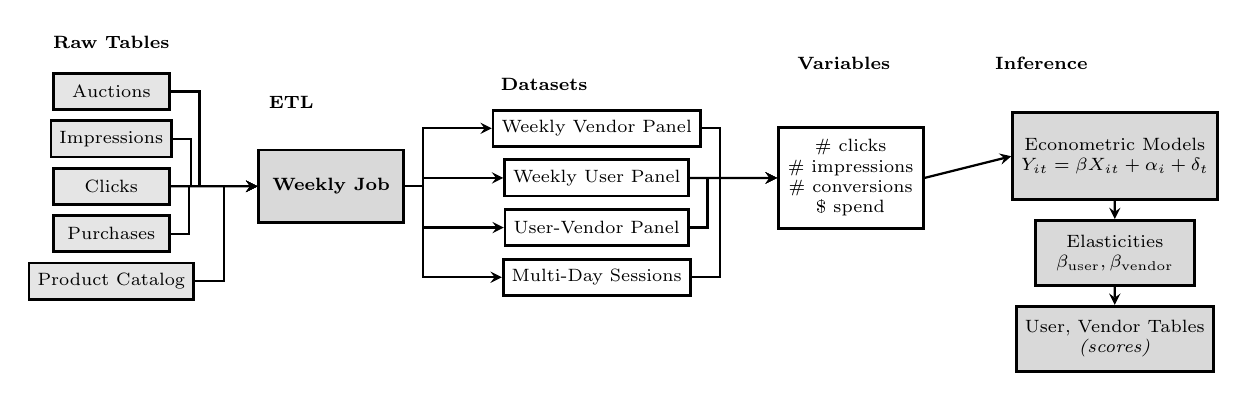
\begin{tikzpicture}[
        scale=0.92, transform shape,
        node distance=0.6cm,
        input/.style={rectangle, minimum width=1.6cm, minimum height=0.5cm, text centered, draw=black, line width=1pt, fill=gray!20, align=center, font=\scriptsize},
        process/.style={rectangle, minimum width=2cm, minimum height=1cm, text centered, draw=black, line width=1pt, fill=gray!30, align=center, font=\scriptsize},
        dataset/.style={rectangle, minimum width=2.4cm, minimum height=0.5cm, text centered, draw=black, line width=1pt, fill=white, align=center, font=\scriptsize},
        varbox/.style={rectangle, minimum width=2cm, minimum height=1.4cm, text centered, draw=black, line width=1pt, fill=white, align=center, font=\scriptsize},
        modelbox/.style={rectangle, minimum width=2.2cm, minimum height=0.6cm, text centered, draw=black, line width=1pt, fill=gray!30, align=center, font=\scriptsize},
        arrow/.style={thick,->,>=stealth}
    ]

        % Level 1: Raw Inputs (5 separate)
        \node (rawheader) [font=\bfseries\scriptsize] {Raw Tables};
        \node (auctions) [input, below=0.2cm of rawheader] {Auctions};
        \node (impressions) [input, below=0.12cm of auctions] {Impressions};
        \node (clicks) [input, below=0.12cm of impressions] {Clicks};
        \node (purchases) [input, below=0.12cm of clicks] {Purchases};
        \node (catalog) [input, below=0.12cm of purchases] {Product Catalog};

        % Level 2: Processing
        \node (etlheader) [right=1.2cm of impressions, yshift=0.5cm, font=\bfseries\scriptsize] {ETL};
        \node (etl) [process, right=1.2cm of clicks] {\textbf{Weekly Job}};

        % Level 3: The Outputs (Fan out)
        \node (datasetsheader) [right=1.2cm of etl, yshift=1.4cm, font=\bfseries\scriptsize] {Datasets};
        \node (vendor) [dataset, right=1.2cm of etl, yshift=0.8cm] {Weekly Vendor Panel};
        \node (user) [dataset, below=0.15cm of vendor] {Weekly User Panel};
        \node (uv) [dataset, below=0.15cm of user] {User-Vendor Panel};
        \node (session) [dataset, below=0.15cm of uv] {Multi-Day Sessions};

        % Level 4: Variables
        \node (varheader) [right=1.2cm of vendor, yshift=0.9cm, font=\bfseries\scriptsize] {Variables};
        \node (vars) [varbox, right=1.2cm of user] {\# clicks \\ \# impressions \\ \# conversions \\ \$ spend};

        % Level 5: Inference
        \node (inferheader) [right=1.2cm of varheader, font=\bfseries\scriptsize] {Inference};
        \node (models) [modelbox, minimum height=1.2cm, right=1.2cm of vars, yshift=0.3cm] {Econometric Models \\ $Y_{it} = \beta X_{it} + \alpha_i + \delta_t$};
        \node (effects) [modelbox, minimum height=0.9cm, below=0.25cm of models] {Elasticities \\ $\beta_{\text{user}}, \beta_{\text{vendor}}$};
        \node (storage) [modelbox, minimum height=0.9cm, below=0.25cm of effects] {User, Vendor Tables \\ \textit{(scores)}};

        % Arrows from inputs to ETL
        \draw [arrow] (auctions.east) -- ++(0.4,0) |- (etl.west);
        \draw [arrow] (impressions.east) -- ++(0.25,0) |- (etl.west);
        \draw [arrow] (clicks.east) -- (etl.west);
        \draw [arrow] (purchases.east) -- ++(0.25,0) |- (etl.west);
        \draw [arrow] (catalog.east) -- ++(0.4,0) |- (etl.west);

        % Arrows from ETL to outputs
        \draw [arrow] (etl.east) -- ++(0.25,0) |- (vendor.west);
        \draw [arrow] (etl.east) -- ++(0.25,0) |- (user.west);
        \draw [arrow] (etl.east) -- ++(0.25,0) |- (uv.west);
        \draw [arrow] (etl.east) -- ++(0.25,0) |- (session.west);

        % Arrows from outputs to variables
        \draw [arrow] (vendor.east) -- ++(0.25,0) |- (vars.west);
        \draw [arrow] (user.east) -- (vars.west);
        \draw [arrow] (uv.east) -- ++(0.25,0) |- (vars.west);
        \draw [arrow] (session.east) -- ++(0.4,0) |- (vars.west);

        % Arrow from variables to inference
        \draw [arrow] (vars.east) -- (models.west);
        \draw [arrow] (models.south) -- (effects.north);
        \draw [arrow] (effects.south) -- (storage.north);

    \end{tikzpicture}

    \vspace{0.3cm}
    \footnotesize
    \textit{Panels}: Repeated observations on same units (users, vendors). \\
    \textit{Multi-Day Shopping Sessions}: Defined by ``inactivity'' windows. \\
    \textit{Econometrics}: Statistical models connecting economic quantities.
\end{frame}

% =============================================================================
% 1. CROSS-SECTIONAL BASELINE
% =============================================================================
\begin{frame}{1. Cross-Sectional Baseline}
    \textbf{Specification:}
    $$ \text{Spend}_{u,v,t} = \alpha + \beta \cdot \text{SponsoredClicks}_{u,v,t} + \epsilon $$
    \footnotesize \textit{$u$ = user, $v$ = vendor, $t$ = week}

    \vspace{0.3cm}
    \begin{itemize}
        \item \textbf{Elasticity:} $\mathbf{+0.22}$ (p=0.08)
    \end{itemize}

    \vfill
    \rule{0.3\textwidth}{0.4pt} \\
    \scriptsize
    \textit{28,619 user-week-vendor cells. 34k clicks, 237 purchases mapped. Mean spend = \$0.22, mean clicks = 1.18.}
\end{frame}

% =============================================================================
% 2a-2b. STAGGERED DID (Callaway-Sant'Anna)
% =============================================================================
\begin{frame}{2a. Ads Drive Exposure but Don't Show Increases in Sales}
    \centering
    \textit{When vendors start advertising, what happens?}
    \vspace{0.2cm}

    \includegraphics[width=0.95\textwidth]{tabfig/event_study_unified_4panel.png}

    \vfill
    \rule{0.4\textwidth}{0.4pt} \\
    \scriptsize
    \textit{Callaway-Sant'Anna (2021). Event study: $\theta(e) = \sum_g w_g \cdot \widehat{ATT}(g, g+e)$. 139k vendors, 26 weeks. Pre-trends passed.}
\end{frame}

\begin{frame}{2b. Premium Vendors Seem to Benefit More}
    \vspace{0.3cm}
    \begin{columns}[t]
        \column{0.48\textwidth}
        \centering
        \textbf{By Adoption Timing}
        \vspace{0.2cm}

        \begin{tabular}{l r l}
            \toprule
            Segment & Effect & 95\% CI \\
            \midrule
            Early (Wk 1-4) & +87\%*** & [72, 102] \\
            Mid (Wk 5-13) & +89\%*** & [80, 98] \\
            Late (Wk 14-26) & +91\%*** & [85, 97] \\
            \bottomrule
        \end{tabular}

        \vspace{0.3cm}
        \footnotesize \textit{No timing advantage}

        \column{0.48\textwidth}
        \centering
        \textbf{By Price Tier}
        \vspace{0.2cm}

        \begin{tabular}{l r l}
            \toprule
            Segment & Effect & 95\% CI \\
            \midrule
            Premium & +0.3\%*** & [0.2, 0.4] \\
            Mid-tier & +0.2\%** & [0.1, 0.3] \\
            Budget & -0.1\% & [-0.3, 0.1] \\
            \bottomrule
        \end{tabular}

        \vspace{0.3cm}
        \footnotesize \textit{Quality signaling}
    \end{columns}

    \vfill
    \rule{0.4\textwidth}{0.4pt} \\
    \scriptsize
    \textit{Effect = \% lift in impressions. TWFE within segments. Timing = week of first ad. Price tier = vendor's median product price quartile.}
\end{frame}

% =============================================================================
% 2c-2d. VENDOR PANEL (TWFE)
% =============================================================================
\begin{frame}{2c. Clicks Associated with an Increase in Sales}
    \textbf{Specification:}
    $$ \ln(Y_{vw}) = \beta \ln(C_{vw}) + \alpha_v + \delta_w + \epsilon_{vw} $$
    \footnotesize \textit{Vendor ($\alpha_v$) and Week ($\delta_w$) FE. SE clustered by vendor.}
    \normalsize

    \vspace{0.3cm}
    \begin{columns}
        \column{0.5\textwidth}
        \begin{itemize}
            \item Elasticity: $\mathbf{+0.64^{***}}$
            \item SE: 0.003, 95\% CI: [0.64, 0.65]
            \item $R^2$ (overall): 0.56
            \item $R^2$ (within): 0.07
        \end{itemize}

        \column{0.5\textwidth}
        \begin{itemize}
            \item Association, not causal
            \item Diminishing returns ($\beta < 1$)
            \item Within-vendor variation
        \end{itemize}
    \end{columns}

    \vfill
    \rule{0.3\textwidth}{0.4pt} \\
    \scriptsize
    \textit{150k vendors, 26 weeks ($N=979k$). $Y$ = revenue, $C$ = clicks. Log-log specification.}
\end{frame}

\begin{frame}{2d. Non-Monotonic Effects: Mid-Tier Sweet Spot}
    \vspace{0.1cm}
    \footnotesize
    \begin{table}
        \centering
        \begin{tabular}{l l r l}
            \toprule
            Dimension & Segment & Effect & Interpretation \\
            \midrule
            \textit{Price} & Premium (>\$82) & 0.00\% & Expensive signal backfires \\
             & Mid-High (\$40-82) & $\mathbf{+0.31\%}$ & Quality signaling sweet spot \\
             & Mid-Low (\$25-40) & -0.08\% & Weak signal \\
             & Budget (<\$25) & -0.10\% & Negative signaling \\
            \midrule
            \textit{Activity} & Medium (Q3) & $\mathbf{+0.76\%}$ & Optimal engagement level \\
             & High (Q4) & +0.39\% & Diminishing returns \\
             & Very High (Q5) & +0.04\% & Saturated \\
            \bottomrule
        \end{tabular}
    \end{table}
    \normalsize

    \vspace{0.2cm}
    \centering
    \textit{Sweet spot = aspirational products with moderate baseline activity.}

    \vfill
    \rule{0.4\textwidth}{0.4pt} \\
    \scriptsize
    \textit{TWFE by segment. Price = vendor median product price quartile. Activity = pre-treatment auction count quartile.}
\end{frame}

% =============================================================================
% 3. USER PANEL (User FE)
% =============================================================================
\begin{frame}{3a. User-Level Panel}
    \textbf{Specification:}
    $$ \ln(Y_{it}) = \beta \ln(C_{it}) + \alpha_i + \delta_t + \epsilon_{it} $$
    \footnotesize \textit{Within-User Variation.}
    \normalsize

    \vspace{0.3cm}
    \begin{columns}
        \column{0.5\textwidth}
        \begin{itemize}
            \item \textbf{Elasticity:} $\mathbf{-0.23^{***}}$
        \end{itemize}

        \column{0.5\textwidth}
        \begin{itemize}
            \item "Comparison Shopping" behavior
        \end{itemize}
    \end{columns}

    \vfill
    \rule{0.3\textwidth}{0.4pt} \\
    \scriptsize
    \textit{9M users, weekly ($N=31M$). FE absorbs time-invariant traits.}
\end{frame}

\begin{frame}{3b. User Heterogeneity}
    \textbf{Mixed Effects:} $\beta_i \sim N(\mu, \sigma^2)$

    \vspace{0.3cm}
    \begin{itemize}
        \item \textbf{Median Effect:} $\mathbf{-0.25}$
        \item \textbf{Variance:} $\mathbf{0.48}$ (High Heterogeneity)
    \end{itemize}

    \vspace{0.3cm}
    \begin{itemize}
        \item \textbf{Browsers:} Negative (comparison mode)
        \item \textbf{Buyers:} Positive (high intent)
    \end{itemize}

    \vfill
    \rule{0.3\textwidth}{0.4pt} \\
    \scriptsize
    \textit{1M user subsample. REML estimation.}
\end{frame}

% =============================================================================
% 4. MICRO-FUNNEL
% =============================================================================
\begin{frame}{4. Micro-Funnel (Journey Level)}
    \textbf{Specification:}
    $$ \ln\left(\frac{P_{ij}}{1-P_{ij}}\right) = \beta C_{ij} + \gamma \mathbf{X}_{ij} $$
    
    \vspace{0.3cm}
    \begin{columns}
        \column{0.5\textwidth}
        \begin{itemize}
            \item \textbf{Elasticity:} $\mathbf{9.25^{***}}$
        \end{itemize}
        
        \column{0.5\textwidth}
        \begin{itemize}
            \item Clicks predict purchase
            \item Inflated by journey intent
        \end{itemize}
    \end{columns}
    
    \vfill
    \rule{0.3\textwidth}{0.4pt} \\
    \scriptsize
    \textit{269k product-journeys. Controls: time, device, category.}
\end{frame}

\begin{frame}{4b. Funnel Heterogeneity}
    \vspace{0.3cm}
    \begin{itemize}
        \item \textbf{New Users:} Effect is \textbf{2x stronger}
        \item \textbf{Loyal Users:} Marginal effect negligible
    \end{itemize}
    
    \vspace{0.3cm}
    \textit{$\Rightarrow$ Ads work for Acquisition, not Retention.}
    
    \vfill
    \rule{0.3\textwidth}{0.4pt} \\
    \scriptsize
    \textit{New User = history $<$ 2 purchases.}
\end{frame}

% Summary Slide\n\\begin{frame}{Elasticities $\\rightarrow$ Products}\n    \\centering\n    \\begin{tabular}{l l}\n        \\toprule\n        \\textbf{Elasticity} & \\textbf{Powers} \\\\\n        \\midrule\n        Vendor-level & Dashboards \\\\\n        User-level & Targeting Engine \\\\\n        Journey/Funnel & Attribution \\\\\n        Cross-vendor & Auction Design \\\\\n        Market-level & GMV Forecasting \\\\\n        \\bottomrule\n    \\end{tabular}\n\\end{frame}

% =============================================================================
% 8. AD RANK --> CLICKS (Muyang)
% =============================================================================
\section{Sponsored Clicks and Ad Rank}

\begin{frame}[plain]
    \vfill
    \centering
    \Huge \textbf{Sponsored Clicks and Ad Rank}
    \vfill
\end{frame}

\begin{frame}{5. Higher-Ranked Ads Associated with Higher CTR}
\[
\mathbb{E}[\text{clicked} \mid \text{rank}]
= \beta_0 - \beta_1 \cdot \text{rank} + \text{controls}.
\]
\vspace{0.8em}

\begin{table}[ht]
\centering
\begin{tabular}{lcccc}
\hline
Method & Baseline OLS & Vendor FE & Vendor + Time FE & DML \\
\hline
Change ($-\beta_1$) & +0.0023pp & +0.0041pp & +0.0036pp & +0.0184pp \\
vs. baseline (2.8\%) & +0.08\% & +0.15\% & +0.13\% & +0.66\% \\
\hline
\end{tabular}
\end{table}

\begin{itemize}
    \item \textbf{Fixed Effect}: Controls for time-invariant unobserved heterogeneity
    \item \textbf{Double Machine Learning}: ML to control confounding while estimating causal effects
\end{itemize}

\vfill
\rule{0.3\textwidth}{0.4pt} \\
\scriptsize
\textit{Rank $\in [1, 50]$ (1 = top). Clicked $\in \{0,1\}$. Unit of observation = 1 ad impression.}

\end{frame}

\begin{frame}{5b. Jump in CTR at Display Cutoffs}
\begin{itemize}
    \item Cutoff at rank 2: 0.189pp, or 6.9\%
\end{itemize}

    \begin{figure}
        \centering
        \includegraphics[width=0.4\linewidth]{tabfig/rdd.png}
    \end{figure}
    \begin{itemize}
        \item Crossing a display cutoff helps ads near the top (e.g., ranks 2 and 4), but hurts ads near the bottom (e.g., ranks 10 and 12)
    \end{itemize}

\vfill
\rule{0.3\textwidth}{0.4pt} \\
\scriptsize
\textit{Display shows 4 ads per row. ``Crossing'' = improving from just below to just above a row boundary (e.g., rank 5 $\rightarrow$ 4 enters row 1). RDD estimates the CTR jump from crossing.}

\end{frame}

\begin{frame}{5c. User Attention Concentrated in Middle Positions}
    \begin{figure}
        \centering
        \includegraphics[width=0.85\linewidth]{tabfig/rankbin.png}
    \end{figure}

    \begin{itemize}
        \item Case 1: Discovery of high-quality products
        \item Case 2: Users avoid first thing they see \& more engaged users scroll deeper
    \end{itemize}

\end{frame}

\begin{frame}{5d. Higher Quality Vendors Less Sensitive to Ranking}

\begin{figure}
    \centering
    \includegraphics[width=0.9\linewidth]{tabfig/vendor.png}
\end{figure}

\begin{itemize}
    \item \textbf{Medium-quality} vendors are most sensitive to ranking position
    \item Suggestion: tailor the ranking to the sensitivity of the vendor
\end{itemize}

\vfill
\rule{0.3\textwidth}{0.4pt} \\
\scriptsize
\textit{High-quality vendors have strong brand recognition or product appeal; they attract clicks regardless of position. N=291 vendors with $\geq$100 impressions across $\geq$3 rank positions.}

\end{frame}

\end{document}
